
\documentclass[10pt,a4paper]{article}

% ===================== PACOTES =====================
\usepackage[brazil]{babel}
\usepackage[utf8]{inputenc}
\usepackage[T1]{fontenc}
\usepackage{geometry}
\geometry{
    a4paper,
    left=3cm,
    right=2cm,
    top=3cm,
    bottom=2.5cm
}

\usepackage{graphicx}
\usepackage{indentfirst}
\usepackage{setspace}
\usepackage{hyperref}
\usepackage{caption}
\usepackage{subcaption}
\usepackage{amsmath,amssymb}
\usepackage{enumitem}
\usepackage{parskip}
\usepackage[expansion=false]{microtype}
\usepackage{fancyhdr}
\usepackage{etoolbox}
\usepackage{listings}
\usepackage{xcolor}
\usepackage{courier}
\usepackage{mathpazo}
\usepackage{float}

% ===================== CÓDIGO R =====================
\definecolor{codebg}{RGB}{245,245,250}
\definecolor{darkgreen}{RGB}{0,100,0}
\definecolor{darkblue}{RGB}{0,0,160}

\lstset{
    language=R,
    basicstyle=\footnotesize\ttfamily,
    keywordstyle=\color{darkblue}\bfseries,
    commentstyle=\color{darkgreen}\itshape,
    stringstyle=\color{red},
    numberstyle=\scriptsize\color{gray},
    backgroundcolor=\color{codebg},
    numbers=none,
    breaklines=true,
    frame=single,
    rulecolor=\color{black!20},
    xleftmargin=12pt,
    xrightmargin=4pt,
    showstringspaces=false,
    tabsize=4,
    captionpos=b,
    abovecaptionskip=6pt,
    literate=
        {á}{{\'a}}1 {à}{{\`a}}1 {ã}{{\~a}}1
        {â}{{\^a}}1 {é}{{\'e}}1 {ê}{{\^e}}1
        {í}{{\'i}}1 {ó}{{\'o}}1 {õ}{{\~o}}1
        {ô}{{\^o}}1 {ú}{{\'u}}1 {ç}{{\c{c}}}1
}

% ===================== CONFIGURAÇÕES =====================
\setlength{\parindent}{1.25cm}
\setlength{\parskip}{0.4em}
\onehalfspacing

\hypersetup{
    colorlinks=true,
    linkcolor=blue,
    urlcolor=blue
}

\captionsetup{
    font=small,
    labelfont=bf
}

% ===================== CABEÇALHO E RODAPÉ =====================
\pagestyle{fancy}
\fancyhf{}

\renewcommand{\headrulewidth}{0.5pt}

\fancyhead[L]{
    
\includegraphics[height=1cm]{imagens/ufc.png}
}

\fancyhead[R]{
    \small{Homework 02 -- Estatística}
}

\renewcommand{\footrulewidth}{0.5pt}

\fancyfoot[C]{\small Estatística para Engenharia}
\fancyfoot[R]{\small\thepage}

\setlength{\headheight}{33pt}

\fancypagestyle{empty}{
    \fancyhf{}
    \renewcommand{\headrulewidth}{0pt}
    \renewcommand{\footrulewidth}{0pt}
}

% ===================== POSICIONAMENTO DE FIGURAS =====================
\renewcommand{\topfraction}{0.95}
\renewcommand{\bottomfraction}{0.95}
\renewcommand{\textfraction}{0.05}
\renewcommand{\floatpagefraction}{0.7}

% ===================== DOCUMENTO =====================
\begin{document}

% ===================== CAPA =====================
\begin{titlepage}
    \centering

    \vspace*{1.5cm}

    
\includegraphics[width=0.35\textwidth]{imagens/ufc.png}\\[1.5cm]

    {\Large\textbf{ESTATÍSTICA PARA ENGENHARIA}}\\[2.5cm]

    {\large
    \textbf{HOMEWORK 02}\\[0.4cm]
    ANÁLISE PROBABILÍSTICA DE SISTEMAS COMPUTACIONAIS
    }

    \vfill

    \begin{flushleft}
        \textbf{ALUNOS:}\\
        ALEXANDRE DE AGUIAR MARTINS GRANGEIRO -- 578345\\
        BRUNO DELUIZ LAGE -- 578342\\
        DANNY SECUNDINO SOUSA FILHO -- 579763\\
        SAULO GOMES PINTO -- 579493\\[0.6cm]

        \textbf{Acesse nosso GitHub:}\\
        \url{https://github.com/dannysecundino/homework-02}
    \end{flushleft}

\end{titlepage}

% ===================== CONTEÚDO =====================

\section{Questão 1}

Esta questão tem o objetivo de modelar o número de requisições que exigem processamento adicional em um lote de requisições de um serviço web, caracterizando a distribuição de probabilidade desse número, calculando suas medidas e algumas probabilidades de interesse e, por fim, estimando por máxima verossimilhança a probabilidade de uma requisição exigir processamento adicional. Diferentemente do Homework 01, não há um conjunto de dados externo: o modelo é definido pelo enunciado e pelo número de matrícula do grupo, e os dados da última parte da questão foram simulados em R. Todo o trabalho computacional foi feito com o R base, sem pacotes externos, utilizando as funções \texttt{dbinom}, \texttt{pbinom}, \texttt{rbinom} e \texttt{optimize}. Em cada ponto, o cálculo teórico foi desenvolvido primeiro e, em seguida, comparado com a saída do código R.

A probabilidade $p$ de uma requisição exigir processamento adicional depende do maior número de matrícula do grupo, $M = 579763$ (variável \texttt{M}):
\[
p = 0{,}05 + \frac{M \bmod 100}{200} = 0{,}05 + \frac{63}{200} = 0{,}05 + 0{,}315 \Rightarrow \boxed{p = 0{,}365}
\]
Logo, $1 - p = 0{,}635$. O tamanho do lote é $n = 50$ requisições, valor comum a todos os grupos.

\subsection{Ponto 1 -- Distribuição de Probabilidade de $X$}

A variável $X$ conta quantas das $n = 50$ requisições do lote exigem processamento adicional. A distribuição binomial é a escolha adequada porque o experimento satisfaz as condições que a definem: o número de tentativas é fixo ($n = 50$); cada requisição tem apenas dois resultados possíveis (exige ou não processamento adicional); as requisições são independentes, conforme o enunciado; e a probabilidade de sucesso $p$ é a mesma para todas elas. Como $X$ é o número de sucessos nessas $n$ tentativas, tem-se
\[
X \sim \text{Bin}(n, p), \qquad \boxed{n = 50, \quad p = 0{,}365}
\]

A função de massa de probabilidade (PMF) é
\[
P(X = x) = \binom{n}{x}\, p^{x}\, (1-p)^{n-x} \Rightarrow 
\]

\[
\boxed{P(X = x) = \binom{50}{x}\, (0{,}365)^{x}\, (0{,}635)^{50-x}} \qquad x \in \{0, 1, 2, \dots, 50\}
\]
e $P(X = x) = 0$ fora desse conjunto. O suporte de $X$ é, portanto, $\{0, 1, \dots, 50\}$: de nenhuma requisição do lote exigindo processamento adicional até todas elas exigindo.

Como verificação, a soma da PMF sobre todo o suporte deve ser igual a 1, o que decorre do teorema binomial, $\sum_{x=0}^{50} \binom{50}{x} p^x (1-p)^{50-x} = (p + (1-p))^{50} = 1$. O código R confirma esse resultado (variável \texttt{sum\_pmf} igual a 1).

\subsection{Ponto 2 -- Gráficos da PMF e da CDF}

Como $X$ é uma variável aleatória discreta, cada função foi representada de forma adequada à sua natureza. A PMF foi desenhada com linhas verticais, já que a probabilidade está concentrada em valores inteiros isolados. A função de distribuição acumulada (CDF), $F(x) = P(X \le x)$, foi desenhada como uma função em escada, que permanece constante entre inteiros consecutivos e dá um salto de tamanho $P(X = x)$ em cada $x$ do suporte.
\begin{figure}[!htb]
\centering
\begin{subfigure}{0.48\textwidth}
    \centering
    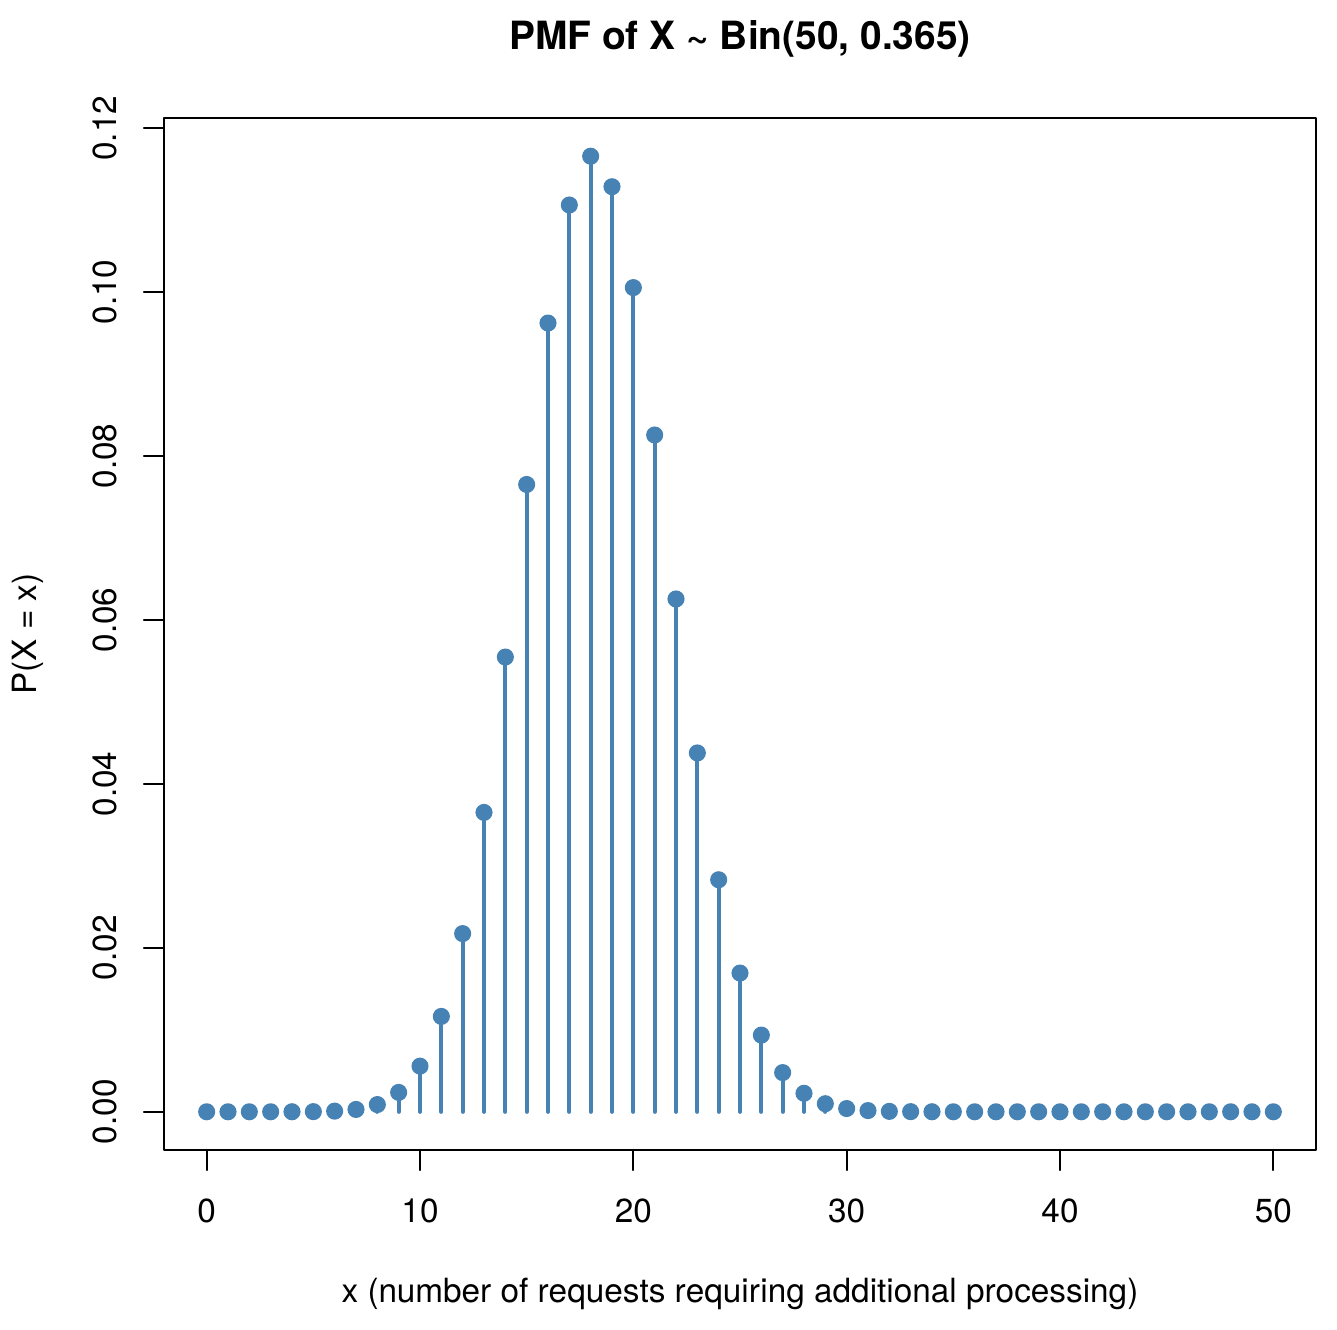
\includegraphics[width=\textwidth]{imagens/pmf_x.png}
    \caption{PMF de $X$}
    \label{fig:q1-pmf}
\end{subfigure}
\hfill
\begin{subfigure}{0.48\textwidth}
    \centering
    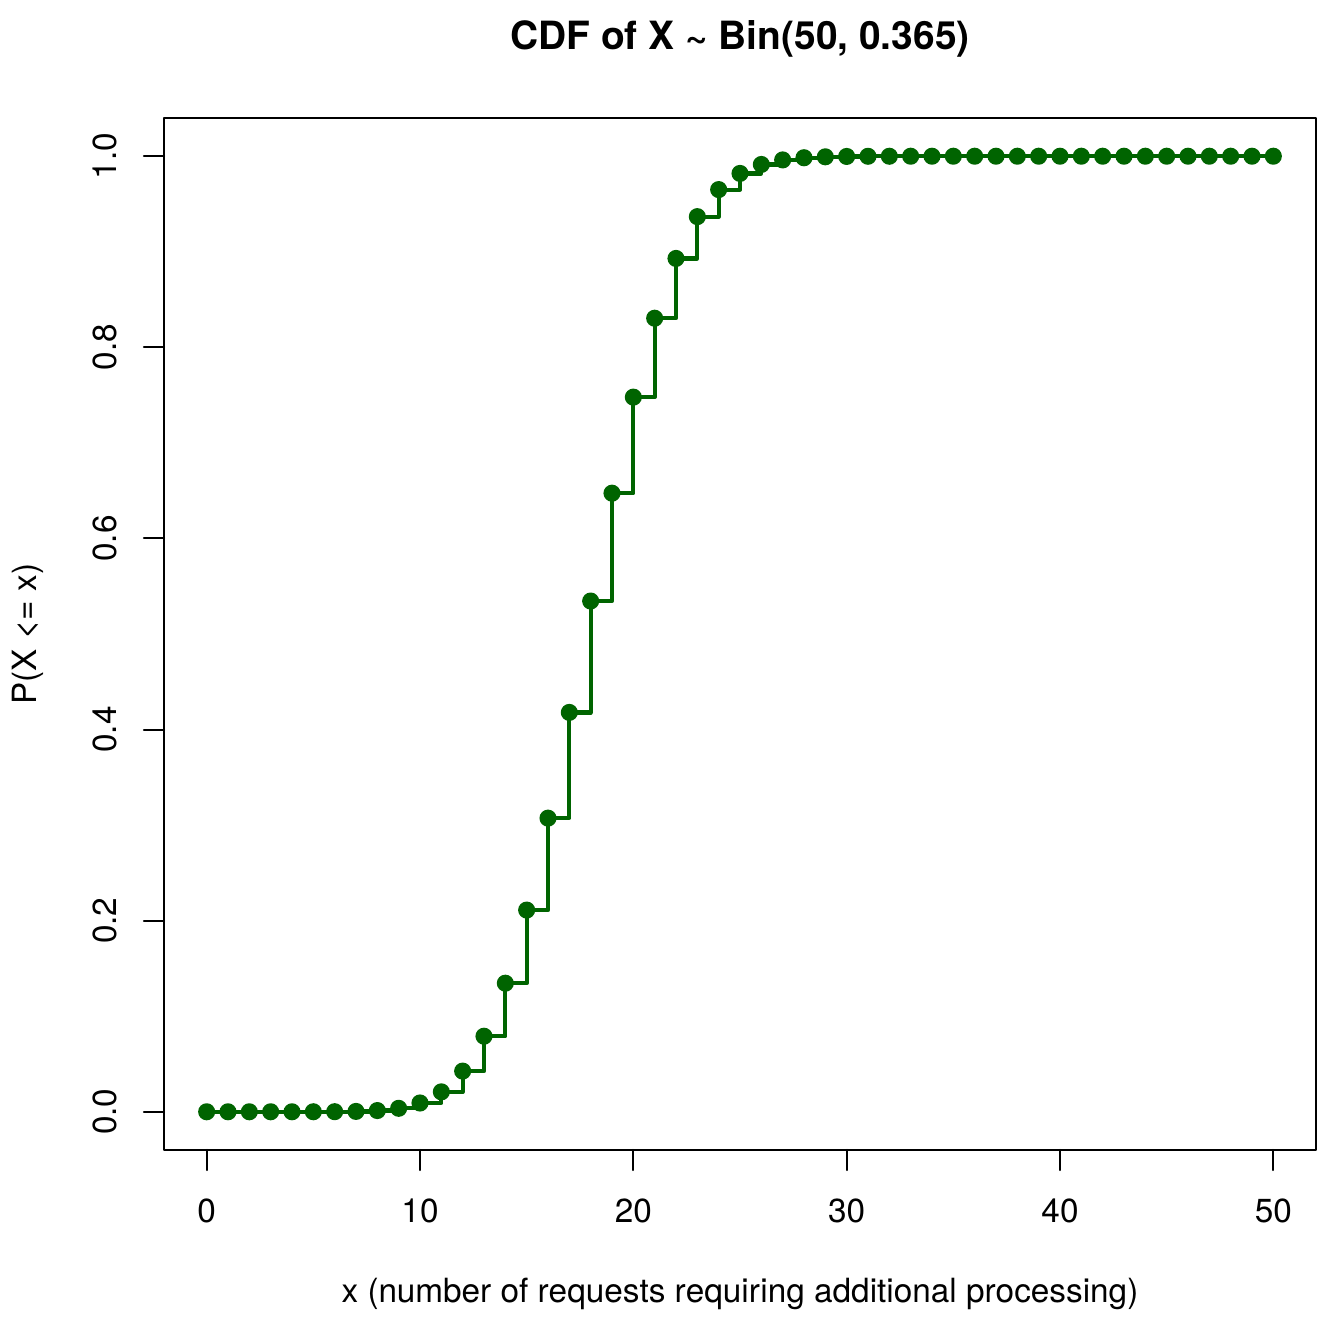
\includegraphics[width=\textwidth]{imagens/cdf_x.png}
    \caption{CDF de $X$}
    \label{fig:q1-cdf}
\end{subfigure}
\caption{PMF e CDF de $X \sim \text{Bin}(50;\, 0{,}365)$}
\label{fig:q1-pmf-cdf}
\end{figure}

A PMF (Figura~\ref{fig:q1-pmf-cdf}a) tem o formato de um sino com pico em $x = 18$, valor com probabilidade $P(X = 18) \approx 0{,}1166$, a maior de todo o suporte (esse valor é a moda da distribuição).

A CDF (Figura~\ref{fig:q1-pmf-cdf}b) parte de valores próximos de zero, cresce com mais rapidez nos degraus da região central e se aproxima de 1 para $x$ acima de 30. Os valores $F(17) \approx 0{,}4179$ e $F(18) \approx 0{,}5345$ mostram que o ponto em que a CDF cruza 0,5 é $x = 18$, de modo que a mediana de $X$ coincide com a moda.

\subsection{Ponto 3 -- Valor Esperado, Variância e Desvio Padrão}

Como X é uma variável binomial, os seguintes resultados podem ser utilizados:
\[
E(X) = n\,p = 50 \cdot 0{,}365 = 18{,}25
\]
\[
\text{Var}(X) = n\,p\,(1-p) = 50 \cdot 0{,}365 \cdot 0{,}635 = 18{,}25 \cdot 0{,}635 = 11{,}58875
\]
\[
\text{DP}(X) = \sqrt{\text{Var}(X)} = \sqrt{11{,}58875} \approx 3{,}4042
\]

Os valores foram conferidos de duas formas no código R: pelas fórmulas fechadas da binomial (variáveis \texttt{ex}, \texttt{vx} e \texttt{sdx}) e pela definição, somando sobre o suporte $\sum_x x\,P(X = x)$ e $\sum_x (x - E(X))^2\,P(X = x)$ (variáveis \texttt{ex\_def}, \texttt{vx\_def} e \texttt{sdx\_def}). As duas formas coincidem com o cálculo teórico, como resume a Tabela~\ref{tab:q1-medidas}.

\begin{table}[H]
\centering
\caption{Medidas de $X \sim \text{Bin}(50;\, 0{,}365)$}
\label{tab:q1-medidas}
\begin{tabular}{lccc}
\hline
\textbf{Medida} & \textbf{Fórmula} & \textbf{Cálculo teórico} & \textbf{Código R} \\
\hline
Valor esperado $E(X)$   & $n\,p$        & 18,25    & 18,25    \\
Variância $\text{Var}(X)$ & $n\,p\,(1-p)$ & 11,58875 & 11,58875 \\
Desvio padrão $\text{DP}(X)$ & $\sqrt{n\,p\,(1-p)}$ & 3,4042 & 3,404225 \\
\hline
\end{tabular}
\end{table}

Isso significa que, em média, cerca de 18 das 50 requisições de um lote exigem processamento adicional (36,5\% do lote, que é o próprio valor de $p$ em porcentagem), com variação típica de aproximadamente 3,4 requisições em torno desse valor.

\subsection{Ponto 4 -- Probabilidades Pedidas}

Como $X$ só assume valores inteiros, cada desigualdade foi reescrita em termos dos inteiros do suporte, e as probabilidades foram expressas pela PMF ou pela CDF, $F(x) = P(X \le x)$.

\paragraph{(a) $P(X \ge 20)$.} Pelo complementar,
\[
P(X \ge 20) = 1 - P(X \le 19) = 1 - F(19) = 1 - \sum_{x=0}^{19} \binom{50}{x}(0{,}365)^{x}(0{,}635)^{50-x}
\]
A soma tem 20 termos e foi avaliada no R, resultando em $F(19) \approx 0{,}6473$ e, portanto, $P(X \ge 20) \approx 1 - 0{,}6473 = 0{,}3527$. O código confirma o valor por dois caminhos independentes, o complementar da CDF e a soma direta da PMF de 20 a 50 (variáveis \texttt{prob\_a} e \texttt{prob\_a\_check}), ambos com $0{,}3526533$. Esse resultado é coerente com o fato de 20 estar logo acima do valor esperado (18,25): em cerca de 35\% dos lotes, 20 ou mais requisições exigiriam processamento adicional.

\paragraph{(b) $P(30 < X < 43)$.} Como $X$ é inteira, $30 < X < 43$ equivale a $31 \le X \le 42$, logo
\[
P(30 < X < 43) = \sum_{x=31}^{42} P(X = x)
\]
Os 12 termos podem ser obtidos à mão pela aplicação direta da pmf
\[
P(X = x) = \binom{n}{x}\, p^{x}\, (1-p)^{n-x}
\]

\begin{table}[H]
\centering
\caption{Termos da soma $P(31 \le X \le 42)$}
\label{tab:q1-termos}
\begin{tabular}{cc|cc}
\hline
$x$ & $P(X = x)$ & $x$ & $P(X = x)$ \\
\hline
31 & $1{,}468 \times 10^{-4}$ & 37 & $6{,}179 \times 10^{-8}$ \\
32 & $5{,}010 \times 10^{-5}$ & 38 & $1{,}215 \times 10^{-8}$ \\
33 & $1{,}571 \times 10^{-5}$ & 39 & $2{,}149 \times 10^{-9}$ \\
34 & $4{,}515 \times 10^{-6}$ & 40 & $3{,}397 \times 10^{-10}$ \\
35 & $1{,}186 \times 10^{-6}$ & 41 & $4{,}763 \times 10^{-11}$ \\
36 & $2{,}841 \times 10^{-7}$ & 42 & $5{,}866 \times 10^{-12}$ \\
\hline
\end{tabular}
\end{table}

A soma dos termos é $P(30 < X < 43) \approx 2{,}187 \times 10^{-4}$, que coincide com o valor do código R, $0{,}000218677$, obtido pela diferença $F(42) - F(30)$ e pela soma direta da PMF (variáveis \texttt{prob\_b} e \texttt{prob\_b\_check}, respectivamente). Observa-se que o primeiro termo responde por cerca de 67\% da soma e que os termos decaem rapidamente, o que é esperado em uma região tão distante do valor esperado: os valores de 31 a 42 situam-se entre 3,7 e 7,0 desvios padrão acima da média. A probabilidade é de aproximadamente 0,022\%.

\paragraph{(c) $P(X = 31)$.} Aplicando a PMF diretamente,
\[
P(X = 31) = \binom{50}{31}(0{,}365)^{31}(0{,}635)^{19}
\]
Com $\binom{50}{31} = \binom{50}{19} = 30\,405\,943\,383\,200 \approx 3{,}0406 \times 10^{13}$ (por simetria do coeficiente binomial), $(0{,}365)^{31} \approx 2{,}6982 \times 10^{-14}$ e $(0{,}635)^{19} \approx 1{,}7894 \times 10^{-4}$, obtém-se
\[
P(X = 31) \approx 3{,}0406 \times 10^{13} \cdot 2{,}6982 \times 10^{-14} \cdot 1{,}7894 \times 10^{-4} \approx 0{,}8204 \cdot 1{,}7894 \times 10^{-4} \approx 1{,}468 \times 10^{-4}
\]
O resultado coincide com o do código R, $0{,}0001468041$ (variáveis \texttt{prob\_c} e \texttt{prob\_c\_check}). Trata-se de uma probabilidade de cerca de 0,015\%, pois 31 está aproximadamente 3,75 desvios padrão acima do valor esperado.

A Tabela~\ref{tab:q1-prob} consolida os resultados deste ponto.

\begin{table}[H]
\centering
\caption{Probabilidades calculadas para $X \sim \text{Bin}(50;\, 0{,}365)$}
\label{tab:q1-prob}
\begin{tabular}{lcc}
\hline
\textbf{Probabilidade} & \textbf{Expressão} & \textbf{Valor} \\
\hline
(a) $P(X \ge 20)$      & $1 - F(19)$       & 0,3527 \\
(b) $P(30 < X < 43)$   & $F(42) - F(30)$   & $2{,}187 \times 10^{-4}$ \\
(c) $P(X = 31)$        & PMF em $x = 31$   & $1{,}468 \times 10^{-4}$ \\
\hline
\end{tabular}
\end{table}

\subsection{Ponto 5 -- Estimação de $p$ por Máxima Verossimilhança}

Nesta parte, supõe-se que $p$ é desconhecido e que se deseja estimá-lo a partir de uma amostra de $n = 50$ requisições independentes, das quais $k$ exigiram processamento adicional. O modelo adotado continua sendo o binomial.

\paragraph{(a) Função de verossimilhança.} A verossimilhança é a própria PMF do modelo, mas vista como função do parâmetro $p$, com o valor observado $k$ fixo:
\[
L(p \mid k) = \binom{50}{k}\, p^{k}\, (1-p)^{50-k}, \qquad 0 < p < 1
\]
Ela mede a plausibilidade de cada valor de $p$ à luz do que foi observado. Se a amostra for tratada como 50 observações de Bernoulli, $x_1, \dots, x_{50}$, com $k = \sum x_i$, a verossimilhança fica $p^{k}(1-p)^{50-k}$, sem o coeficiente binomial. Como esse coeficiente não depende de $p$, ele não altera o ponto de máximo, e o estimador obtido é o mesmo nos dois casos.

\paragraph{(b) Log-verossimilhança e estimador de máxima verossimilhança.} Como o logaritmo é crescente, maximizar $L$ é equivalente a maximizar $\ell(p) = \ln L(p \mid k)$, que é mais simples de derivar porque transforma o produto em soma:
\[
\ell(p) = \ln\binom{50}{k} + k \ln p + (50 - k)\ln(1-p)
\]
Derivando em relação a $p$ e igualando a zero,
\[
\ell'(p) = \frac{k}{p} - \frac{50-k}{1-p} = 0 \;\Longrightarrow\; k(1-p) = (50-k)\,p \;\Longrightarrow\; k - kp = 50p - kp \;\Longrightarrow\; \boxed{\hat{p} = \frac{k}{50}}
\]
O termo $\ln\binom{50}{k}$ desaparece na derivada, por não depender de $p$. Para confirmar que o ponto crítico é um máximo, calcula-se a segunda derivada,
\[
\ell''(p) = -\frac{k}{p^{2}} - \frac{50-k}{(1-p)^{2}} < 0, \qquad 0 < p < 1 \;\; (0 < k < 50)
\]
que é negativa em todo o intervalo. O estimador de máxima verossimilhança é, portanto, a proporção amostral de requisições que exigiram processamento adicional.

\paragraph{(c) Amostra simulada e estimativa.} Foi gerada uma amostra de 50 observações i.i.d. de Bernoulli com a probabilidade teórica $p = 0{,}365$, utilizando \texttt{rbinom(n, size = 1, prob = p)} (uma Bernoulli é uma binomial com uma única tentativa) e a semente fixa \texttt{set.seed(M)}, para que o resultado seja reproduzível. Na amostra gerada, observou-se
\[
k = 14 \quad \Longrightarrow \quad \hat{p} = \frac{k}{n} = \frac{14}{50} = 0{,}28
\]
A estimativa também foi obtida numericamente, maximizando a log-verossimilhança com a função \texttt{optimize} (variável \texttt{p\_hat\_num}), o que resultou em $0{,}2800024$. A pequena diferença de cerca de $2 \times 10^{-6}$ em relação a $0{,}28$ decorre da tolerância do otimizador, e o resultado confirma a dedução do item (b). A segunda derivada no ponto de máximo vale $\ell''(0{,}28) = -\frac{14}{0{,}28^2} - \frac{36}{0{,}72^2} \approx -178{,}57 - 69{,}44 = -248{,}02 < 0$, confirmando que se trata de um máximo.

A Figura~\ref{fig:q1-lik} mostra a função de verossimilhança para $k = 14$. A curva tem um único pico em $\hat{p} = 0{,}28$, com valor $L(0{,}28 \mid 14) \approx 0{,}1248$. Já o valor teórico $p = 0{,}365$ tem verossimilhança $L(0{,}365 \mid 14) \approx 0{,}0555$, cerca de 44\% da máxima: os dados observados não descartam o valor teórico, mas são mais compatíveis com um valor menor.

\begin{figure}[H]
\centering
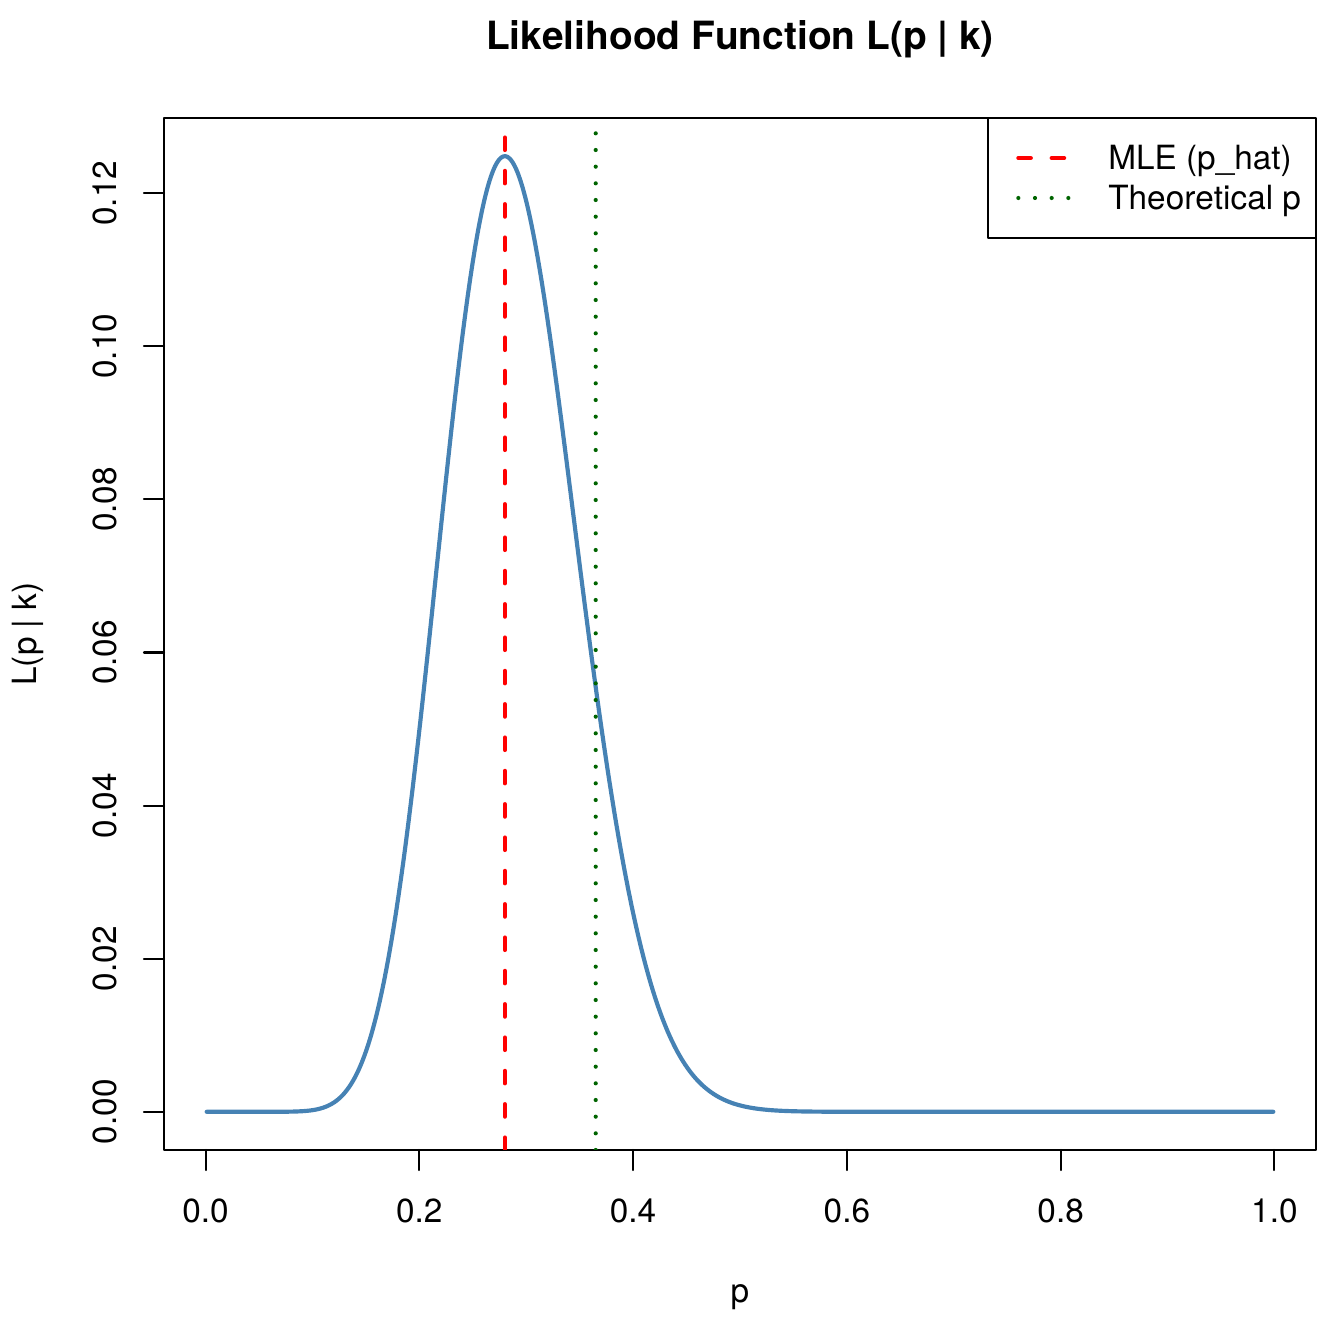
\includegraphics[width=0.5\textwidth]{imagens/likelihood_p.png}
\caption{Função de verossimilhança $L(p \mid k = 14)$, com a estimativa de máxima verossimilhança $\hat{p}$ e a probabilidade teórica $p$ marcadas}
\label{fig:q1-lik}
\end{figure}

\paragraph{(d) Comparação com a probabilidade teórica.} A estimativa $\hat{p} = 0{,}28$ difere da probabilidade teórica $p = 0{,}365$ em $0{,}085$ (diferença absoluta), o que equivale a cerca de 23\% do valor teórico. Essa diferença é esperada em uma amostra finita por três razões.

A primeira é que $\hat{p} = k/n$ é uma variável aleatória, pois $k$ muda de amostra para amostra mesmo com $p$ fixo. O estimador é não viesado, $E(\hat{p}) = E(k)/n = np/n = p$, ou seja, acerta $p$ em média, mas cada amostra individual flutua em torno dele, com variância e erro padrão dados por
\[
\text{Var}(\hat{p}) = \frac{n\,p\,(1-p)}{n^{2}} = \frac{p(1-p)}{n}, \qquad \text{EP}(\hat{p}) = \sqrt{\frac{p(1-p)}{n}} = \sqrt{\frac{0{,}365 \cdot 0{,}635}{50}} \approx 0{,}0681
\]
Assim, a diferença observada de $0{,}085$ corresponde a cerca de $0{,}085/0{,}0681 \approx 1{,}25$ erros padrão, uma distância comum de ocorrer por acaso. De fato, sob $p = 0{,}365$, a probabilidade de observar $k \le 14$ em 50 requisições é $P(X \le 14) \approx 0{,}1346$, de modo que obter 14 ou menos não é um evento raro.

A segunda razão é que, com $n = 50$, $\hat{p}$ só pode assumir múltiplos de $1/50 = 0{,}02$, de modo que o valor exato $0{,}365$ nem sequer pode ser atingido; os valores mais próximos seriam $0{,}36$ e $0{,}38$.

A terceira é a variabilidade amostral em si, que depende do tamanho da amostra, como mostra o erro padrão: ele é proporcional a $1/\sqrt{n}$, de modo que aumentar a amostra reduz a dispersão de $\hat{p}$ em torno de $p$. Para ilustrar esse efeito, o código gerou amostras de Bernoulli de tamanhos crescentes, com o mesmo $p$, e calculou $\hat{p}$ e o erro padrão teórico em cada caso (Tabela~\ref{tab:q1-tamanho}).

\begin{table}[H]
\centering
\caption{Efeito do tamanho amostral sobre a estimativa de $p$ ($p = 0{,}365$)}
\label{tab:q1-tamanho}
\begin{tabular}{rcccc}
\hline
$n$ & $\hat{p}$ & $|\hat{p} - p|$ & $\text{EP}(\hat{p})$ & $|\hat{p} - p|/\text{EP}(\hat{p})$ \\
\hline
10     & 0,40000 & 0,03500 & 0,1522 & 0,23 \\
50     & 0,38000 & 0,01500 & 0,0681 & 0,22 \\
500    & 0,36200 & 0,00300 & 0,0215 & 0,14 \\
5\,000  & 0,36940 & 0,00440 & 0,0068 & 0,65 \\
50\,000 & 0,36846 & 0,00346 & 0,0022 & 1,61 \\
\hline
\end{tabular}
\end{table}

Duas observações são necessárias sobre a tabela. Primeiro, a linha $n = 50$ corresponde a uma nova amostra, gerada em sequência no código, e por isso é diferente da amostra com $k = 14$ usada nos itens anteriores. Segundo, o erro padrão cai de forma sistemática com o aumento de $n$ (a cada multiplicação do tamanho por 10, ele diminui por um fator de $\sqrt{10} \approx 3{,}16$, de $0{,}0681$ para $0{,}0215$, $0{,}0068$ e $0{,}0022$), mas o erro observado em cada amostra individual não diminui de forma estritamente monótona, pois cada amostra é um sorteio: o erro em $n = 5\,000$ ($0{,}0044$) é maior que em $n = 500$ ($0{,}0030$). O que se verifica é que todos os erros ficaram dentro de dois erros padrão. Esse comportamento ilustra a consistência do estimador, isto é, $\hat{p}$ se aproxima de $p$ à medida que o tamanho da amostra aumenta, conforme a Lei dos Grandes Números.
\clearpage

\section{Questão 2}

Esta questão tem o objetivo de modelar o número diário de alertas críticos gerados pelo serviço web a partir dos resultados da Questão 1, aproximar a distribuição exata desse número por 
uma distribuição de Poisson e avaliar a qualidade dessa aproximação, tanto de forma analítica quanto por simulação. Assim como na Questão 1, não há conjunto de dados externo: o modelo 
é definido pelo enunciado em função de $m = E(X)$ e $c = \text{DP}(X)$, e os dados do último ponto foram simulados em R. Foi utilizado apenas o R base, com as funções \texttt{dbinom}, 
\texttt{dpois}, \texttt{rbinom} e \texttt{barplot}. Em cada ponto, o cálculo teórico foi desenvolvido primeiro e, em seguida, comparado com a saída do código R.

Os valores obtidos na Questão 1 são
\[
m = E(X) = 18{,}25, \qquad c = \text{DP}(X) = \sqrt{11{,}58875} \approx 3{,}4042
\]

\subsection{Ponto 1 -- Cálculo de $N$ e $p_{\text{alerta}}$ e Aproximação de Poisson}

O número de requisições por dia e a probabilidade de uma requisição gerar um alerta crítico são
\[
N = \text{round}(m \times 10^{6}) = \text{round}(18{,}25 \times 10^{6}) \Rightarrow \boxed{N = 18\,250\,000}
\]
\[
p_{\text{alerta}} = \frac{c}{N} = \frac{3{,}4042}{18\,250\,000} \Rightarrow \boxed{p_{\text{alerta}} \approx 1{,}8653 \times 10^{-7}}
\]

A variável $Y$ conta quantas das $N$ requisições do dia geram um alerta crítico. Como o número de tentativas é fixo, cada requisição tem dois resultados possíveis, as requisições são 
independentes e a probabilidade $p_{\text{alerta}}$ é a mesma para todas, a distribuição exata de $Y$ é binomial:
\[
Y \sim \text{Bin}(N, p_{\text{alerta}}), \qquad P(Y = y) = \binom{N}{y}\, p_{\text{alerta}}^{\,y}\, (1 - p_{\text{alerta}})^{N-y}, \quad y \in \{0, 1, \dots, N\}
\]

Com $N$ muito grande e $p_{\text{alerta}}$ muito pequeno, o cálculo direto dessa PMF é inviável à mão, e a distribuição binomial pode ser aproximada por uma distribuição de Poisson 
(lei dos eventos raros), cujo parâmetro é o valor esperado de $Y$:
\[
\lambda = N\,p_{\text{alerta}} = c \approx 3{,}4042 \qquad \Rightarrow \qquad Y \approx \text{Pois}(\lambda)
\]
A PMF da aproximação e o seu suporte são
\[
\boxed{P(Y = y) = \frac{e^{-\lambda}\,\lambda^{y}}{y!} = \frac{e^{-3{,}4042}\,(3{,}4042)^{y}}{y!}}, \qquad y \in \{0, 1, 2, \dots\}
\]

\paragraph{Adequação da aproximação.} A aproximação é adequada quando $N$ é grande, $p_{\text{alerta}}$ é pequeno e $\lambda = N\,p_{\text{alerta}}$ é moderado. As três condições são 
satisfeitas: $N = 1{,}825 \times 10^{7}$, $p_{\text{alerta}} \approx 1{,}87 \times 10^{-7}$ e $\lambda \approx 3{,}40$. A Tabela~\ref{tab:q2-pmf} compara as duas PMFs nos primeiros 
valores do suporte, calculadas com \texttt{dbinom} e \texttt{dpois}.

\begin{table}[H]
\centering
\caption{PMF exata (binomial) e aproximada (Poisson) de $Y$}
\label{tab:q2-pmf}
\begin{tabular}{cccc}
\hline
$y$ & \textbf{Binomial} & \textbf{Poisson} & \textbf{Diferença absoluta} \\
\hline
0 & 0,033232544 & 0,033232555 & $1{,}06 \times 10^{-8}$ \\
1 & 0,113131090 & 0,113131105 & $1{,}48 \times 10^{-8}$ \\
2 & 0,192561885 & 0,192561885 & $1{,}5 \times 10^{-10}$ \\
3 & 0,218508032 & 0,218508015 & $1{,}70 \times 10^{-8}$ \\
4 & 0,185962647 & 0,185962629 & $1{,}86 \times 10^{-8}$ \\
5 & 0,126611746 & 0,126611738 & $8{,}5 \times 10^{-9}$ \\
6 & 0,071835812 & 0,071835814 & $1{,}5 \times 10^{-9}$ \\
\hline
\end{tabular}
\end{table}

Para $y = 0, \dots, 20$ (variável \texttt{max\_abs\_diff}), a maior diferença absoluta entre as duas PMFs é de apenas $1{,}86 \times 10^{-8}$, observada em $y = 4$, e a maior diferença 
relativa é de cerca de $7 \times 10^{-6}$. Os resultados indicam que as duas distribuições são praticamente indistinguíveis neste caso, de modo que a Poisson, que depende de um único 
parâmetro e é muito mais simples de calcular, representa bem o comportamento de $Y$. Uma diferença estrutural é que o suporte da Poisson é ilimitado, enquanto o da binomial termina em 
$N$; contudo, a probabilidade atribuída a valores muito acima da média é desprezível nos dois modelos.

\subsection{Ponto 2 -- Valor Esperado e Variância de $Y$}

Para a distribuição exata, $Y \sim \text{Bin}(N, p_{\text{alerta}})$, e para a aproximação, $Y \approx \text{Pois}(\lambda)$, tem-se
\[
\text{Exata:} \quad E(Y) = N\,p_{\text{alerta}} = 3{,}404225316
\]
\[
\text{Exata:} \quad \text{Var}(Y) = N\,p_{\text{alerta}}\,(1 - p_{\text{alerta}}) \approx 3{,}404224681
\]
\[
\text{Poisson:} \quad E(Y) = \text{Var}(Y) = \lambda = 3{,}404225316
\]

Os valores foram conferidos no código R de duas formas: pelas fórmulas fechadas (variáveis \texttt{ey\_exact}, \texttt{vy\_exact}, \texttt{ey\_pois} e \texttt{vy\_pois}) e pela 
definição, somando sobre $y = 0, \dots, 100$, já que a probabilidade além desse valor é desprezível (variáveis com sufixo \texttt{\_check}). As duas formas coincidem com o cálculo 
teórico, como resume a Tabela~\ref{tab:q2-medidas}.

\begin{table}[H]
\centering
\caption{Valor esperado e variância de $Y$: distribuição exata e aproximação de Poisson}
\label{tab:q2-medidas}
\begin{tabular}{lccc}
\hline
\textbf{Medida} & \textbf{Exata (binomial)} & \textbf{Poisson} & \textbf{Diferença} \\
\hline
$E(Y)$   & 3,404225316 & 3,404225316 & 0 \\
$\text{Var}(Y)$ & 3,404224681 & 3,404225316 & $6{,}35 \times 10^{-7}$ \\
\hline
\end{tabular}
\end{table}

Os valores esperados são idênticos, pois ambas as distribuições são parametrizadas de modo que $E(Y) = N\,p_{\text{alerta}}$. As variâncias diferem pelo fator $(1 - p_{\text{alerta}})$, 
presente apenas na binomial: a diferença absoluta é $N\,p_{\text{alerta}}^{2} = c\,p_{\text{alerta}} \approx 6{,}35 \times 10^{-7}$ e a diferença relativa é igual a 
$p_{\text{alerta}} \approx 1{,}87 \times 10^{-7}$ (variável \texttt{rel\_diff\_v}), isto é, cerca de $0{,}00002\%$. Como $p_{\text{alerta}}$ é muito pequeno, $1 - p_{\text{alerta}} \approx 1$, 
e a binomial se comporta como uma Poisson, cuja variância é igual à média. Em termos práticos, o serviço gera em média cerca de 3,4 alertas críticos por dia, com variação típica de 
aproximadamente $\sqrt{3{,}4042} \approx 1{,}85$ alertas em torno desse valor, e qualquer um dos dois modelos fornece essa conclusão.

\subsection{Ponto 3 -- Simulação de 10.000 Dias de Operação}

Foram simulados $10\,000$ dias de operação a partir da distribuição binomial exata, utilizando \texttt{rbinom(10000, size = N, prob = p\_alert)} com a semente fixa \texttt{set.seed(M)}, 
para que o resultado seja reproduzível. Cada valor simulado é o número de alertas críticos de um dia. Os valores observados variaram de 0 a 15 alertas por dia. A Figura~\ref{fig:q2-sim} 
compara as frequências relativas observadas com a PMF da Poisson.

\begin{figure}[H]
\centering
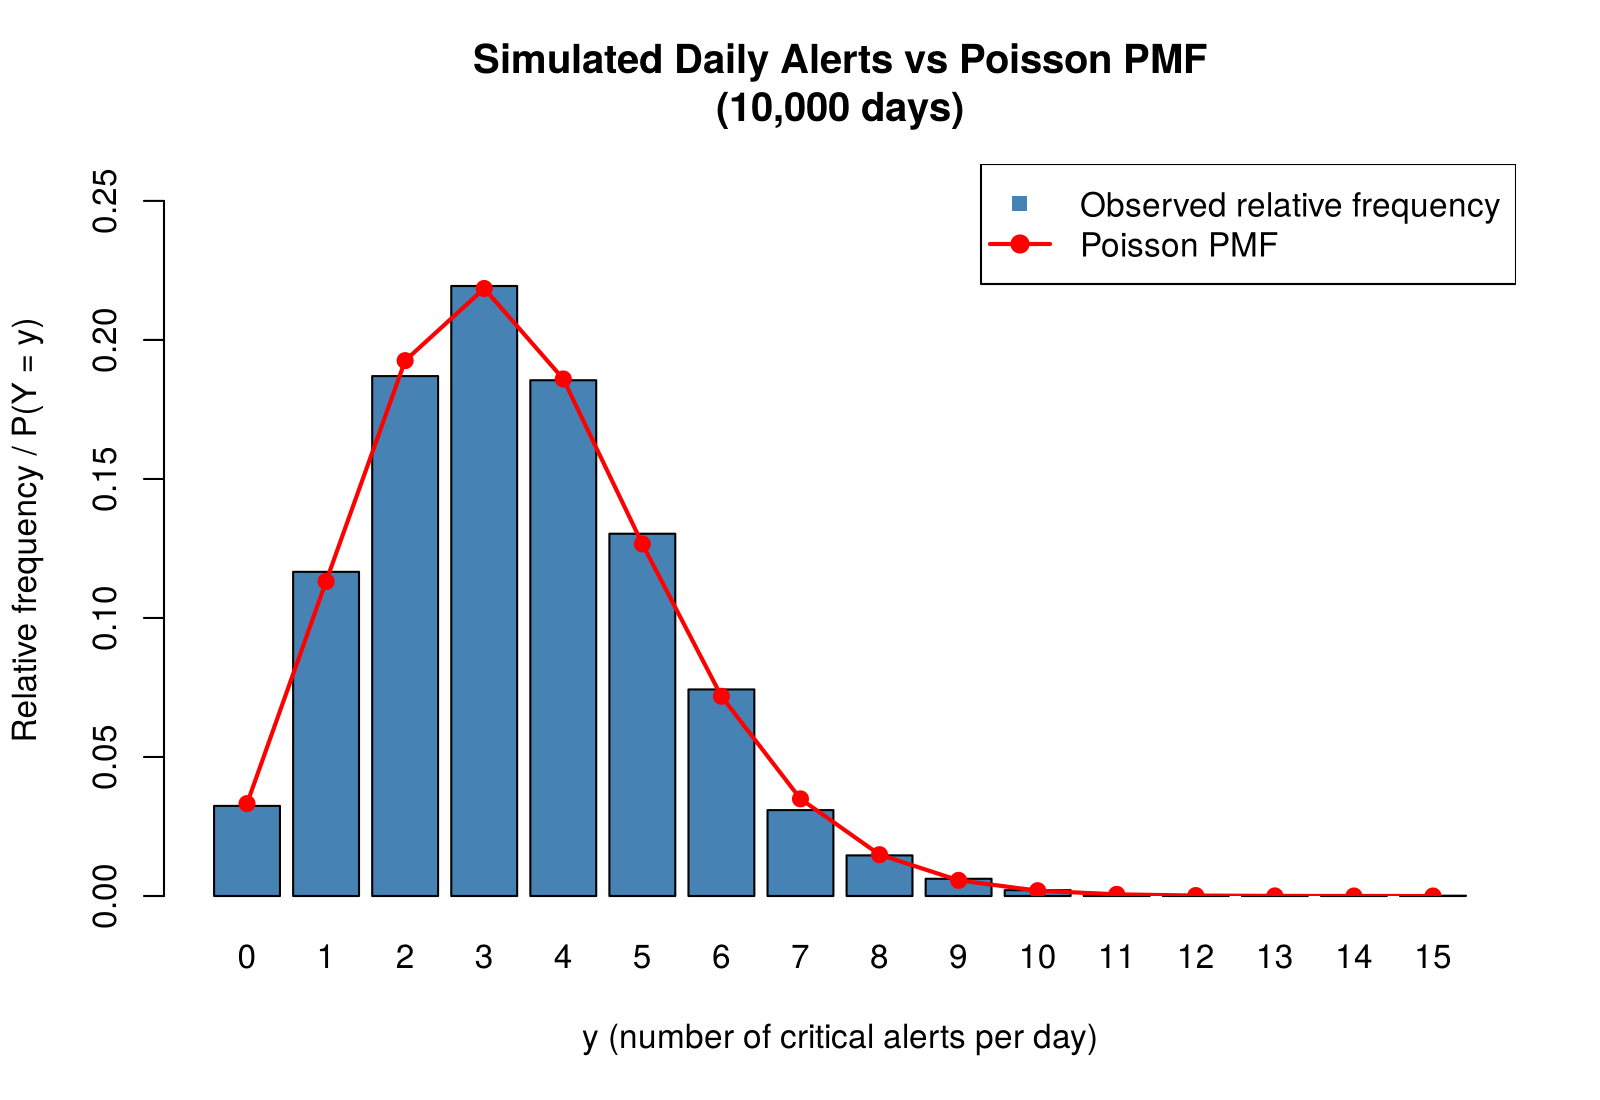
\includegraphics[width=0.75\textwidth]{imagens/sim_poisson_q2.png}
\caption{Frequências relativas do número diário de alertas em 10.000 dias simulados (barras) e PMF da distribuição de Poisson com $\lambda = 3{,}4042$ (pontos e linha)}
\label{fig:q2-sim}
\end{figure}

O gráfico mostra que as frequências observadas acompanham de perto a PMF da Poisson: a distribuição é unimodal, com moda em $y = 3$ (frequência de 0,2194 contra 0,2185 teórico) e assimetria 
à direita, e a cauda se extingue de forma semelhante nas duas representações.

A qualidade da aproximação foi avaliada por três medidas, apresentadas na Tabela~\ref{tab:q2-qualidade}.

\begin{table}[H]
\centering
\caption{Comparação entre a simulação (10.000 dias) e a distribuição de Poisson}
\label{tab:q2-qualidade}
\begin{tabular}{lcc}
\hline
\textbf{Medida} & \textbf{Simulação} & \textbf{Teórico ($\lambda = 3{,}4042$)} \\
\hline
Média amostral         & 3,4064 & 3,4042 \\
Variância amostral     & 3,3996 & 3,4042 \\
Maior diferença entre frequência e PMF & 0,0056 (em $y = 2$) & -- \\
\hline
\end{tabular}
\end{table}

A média e a variância amostrais ficaram muito próximas de $\lambda$, o que é coerente com a propriedade de a Poisson ter média igual à variância. O erro padrão da média amostral é 
$\sqrt{\lambda/10\,000} \approx 0{,}0185$, de modo que a diferença de $0{,}0022$ equivale a cerca de $0{,}12$ erro padrão. A maior diferença entre uma frequência relativa e a PMF 
correspondente foi de $0{,}0056$, em $y = 2$ (frequência de $0{,}1870$ contra $0{,}1926$). Para comparação, o erro padrão de uma frequência relativa no valor mais provável da distribuição 
($P(Y = 3) \approx 0{,}2185$) é $\sqrt{0{,}2185\,(1 - 0{,}2185)/10\,000} \approx 0{,}0041$ (variável \texttt{se\_freq}), de modo que a maior diferença corresponde a cerca de $1{,}3$ erro 
padrão, ou seja, é compatível com a variabilidade aleatória da simulação. Nas caudas, os valores $y = 14$ e $y = 15$ foram observados uma vez cada, embora suas probabilidades teóricas 
sejam $1{,}07 \times 10^{-5}$ e $2{,}43 \times 10^{-6}$ (cerca de 0,11 e 0,02 dia esperado em 10.000 dias); trata-se de eventos raros cuja ocorrência isolada gera diferenças da ordem de 
$10^{-4}$, sem relevância prática.

Os resultados indicam que a aproximação de Poisson descreve bem o número diário de alertas. É importante observar, entretanto, o alcance dessa conclusão: a diferença entre a binomial 
exata e a Poisson (no máximo $1{,}86 \times 10^{-8}$ por valor, conforme o Ponto 1) é cerca de cinco ordens de grandeza menor que o ruído de uma simulação de 10.000 dias 
($\approx 4 \times 10^{-3}$). Assim, a simulação não consegue distinguir as duas distribuições, e seria necessária uma amostra da ordem de $10^{14}$ dias para que o erro padrão se tornasse 
comparável àquela diferença. A simulação confirma, portanto, a coerência do modelo com a Poisson, enquanto a qualidade da aproximação em si é estabelecida pela comparação analítica das PMFs 
e dos momentos (Pontos 1 e 2).
\clearpage

\section{Questão 3}

Esta questão tem o objetivo de modelar a temperatura da CPU sob condições normais de operação como uma variável aleatória contínua normalmente distribuída, implementar em R um gerador de valores normais a partir da transformação de Box-Muller, compará-lo ao gerador nativo da linguagem, determinar uma temperatura crítica associada aos resultados da Questão~1 e avaliar, numérica e visualmente, o ajuste dos dados simulados à distribuição teórica. Assim como nas questões anteriores, não há conjunto de dados externo: o modelo é especificado pelo enunciado, com média $\mu = 62\,^\circ\text{C}$ e desvio padrão $\sigma = 3{,}5\,^\circ\text{C}$, isto é, $T \sim N(62;\; 3{,}5^{2})$, e os dois conjuntos de temperaturas são simulados em R com tamanho determinado pelo valor esperado $m = E(X)$ obtido na Questão~1. Todo o processamento foi realizado apenas com o R base, sem pacotes externos, utilizando as funções \texttt{runif}, \texttt{rnorm}, \texttt{pbinom}, \texttt{qnorm}, \texttt{pnorm}, \texttt{dnorm}, \texttt{hist} e \texttt{set.seed}. Em cada ponto, os resultados teóricos são estabelecidos primeiro e, em seguida, comparados aos valores obtidos computacionalmente.

\subsection{Ponto 1 -- Implementação da Transformação de Box-Muller}

O número de temperaturas da CPU a simular, $n_T$, depende do valor esperado $m = E(X) = 18{,}25$ calculado na Questão~1:
\[
n_T = \text{round}(100\,m) = \text{round}(100 \cdot 18{,}25) \;\Longrightarrow\; \boxed{n_T = 1\,825}
\]

A transformação de Box-Muller permite gerar variáveis aleatórias normais padrão independentes a partir de variáveis uniformes independentes em $(0, 1)$, explorando a representação em coordenadas polares de um par $(Z_1, Z_2)$ normal bivariado padrão (em que o raio ao quadrado $R^{2} = Z_1^{2} + Z_2^{2}$ segue distribuição exponencial de taxa $1/2$ e o ângulo $\Theta$ é uniforme em $[0, 2\pi)$). O procedimento implementado na função \texttt{box\_muller(n, mu = 0, sigma = 1)} executa as três etapas especificadas:
\begin{enumerate}[label=(\alph*)]
    \item \textbf{Geração de uniformes independentes:} geram-se pares $U_1, U_2 \sim \text{Unif}(0, 1)$ independentes por meio da função \texttt{runif}. No R, \texttt{runif} não retorna exatamente $0$ nem $1$, de modo que $\ln(U_1)$ é sempre finito e bem definido.
    \item \textbf{Cálculo das variáveis normais padrão:} para cada par $(U_1, U_2)$, calculam-se duas variáveis aleatórias independentes com distribuição $N(0, 1)$:
    \[
    Z_1 = \sqrt{-2 \ln(U_1)}\,\cos(2\pi U_2), \qquad Z_2 = \sqrt{-2 \ln(U_1)}\,\sin(2\pi U_2)
    \]
    Como cada par produz dois valores normais padrão, para obter $n_T = 1\,825$ observações são necessários $\lceil n_T / 2 \rceil = \lceil 1\,825 / 2 \rceil = 913$ pares, resultando em $2 \times 913 = 1\,826$ valores. Os vetores \texttt{z1} e \texttt{z2} são concatenados em um único vetor \texttt{z} e truncados ao comprimento exato \texttt{z[1:n]}, descartando o único valor excedente.
    \item \textbf{Conversão para temperaturas da CPU:} por fim, aplica-se a transformação linear de locação e escala
    \[
    \boxed{T = \mu + \sigma Z = 62 + 3{,}5\,Z}
    \]
    Como $Z \sim N(0, 1)$, segue das propriedades da distribuição normal que $E(T) = 62 + 3{,}5\,E(Z) = 62\,^\circ\text{C}$ e $\text{Var}(T) = 3{,}5^{2}\,\text{Var}(Z) = 12{,}25\,^\circ\text{C}^{2}$, isto é, $T \sim N(62;\; 3{,}5^{2})$. Com os argumentos padrão \texttt{mu = 0} e \texttt{sigma = 1}, a função devolve valores normais padrão; quando chamada com \texttt{mu = 62} e \texttt{sigma = 3.5}, devolve diretamente as temperaturas simuladas.
\end{enumerate}

\subsection{Ponto 2 -- Geração dos Conjuntos de Dados Simulados}

Para garantir a reprodutibilidade dos experimentos e, ao mesmo tempo, preservar a independência estatística entre as duas amostras, definiu-se uma única semente aleatória fixa antes da geração de ambos os conjuntos (\texttt{set.seed(M)}, com $M = 579763$), gerando os dois vetores sequencialmente:
\begin{itemize}
    \item \textbf{Conjunto 1 (\texttt{temp\_bm}):} $n_T = 1\,825$ temperaturas geradas pela função \texttt{box\_muller}, invocada com \texttt{mu = 62} e \texttt{sigma = 3.5};
    \item \textbf{Conjunto 2 (\texttt{temp\_r}):} $n_T = 1\,825$ temperaturas geradas imediatamente em seguida pela função nativa \texttt{rnorm} do R, com os mesmos parâmetros (que, por padrão, emprega o método da inversão sobre o gerador Mersenne-Twister).
\end{itemize}

Por consumirem trechos disjuntos da mesma sequência pseudoaleatória, os dois conjuntos são amostras independentes de $N(62;\; 3{,}5^{2})$. Como verificação inicial no código, confirmou-se que ambos possuem comprimento exato igual a $1\,825$ (variáveis \texttt{len\_bm} e \texttt{len\_r}), com médias amostrais de $61{,}9283\,^\circ\text{C}$ (Box-Muller) e $62{,}0000\,^\circ\text{C}$ (\texttt{rnorm}) e desvios padrão amostrais de $3{,}5269\,^\circ\text{C}$ e $3{,}5549\,^\circ\text{C}$, valores próximos aos parâmetros teóricos $\mu = 62\,^\circ\text{C}$ e $\sigma = 3{,}5\,^\circ\text{C}$.

\subsection{Ponto 3 -- Temperatura Crítica $T_{\text{crit}}$ e Análise dos Conjuntos Simulados}

\paragraph{Cálculo teórico de $r$ e de $T_{\text{crit}}$.} Na Questão~1, $X \sim \text{Bin}(50;\; 0{,}365)$ tem valor esperado $m = E(X) = 18{,}25$. Como $X$ assume apenas valores inteiros, o evento $X \ge 18{,}25$ equivale a $X \ge 19$, logo
\[
r = P(X \ge E(X)) = P(X \ge 19) = 1 - P(X \le 18) = 1 - F(18)
\]
Utilizando $F(18) \approx 0{,}534495$ (já observado na análise da CDF da Questão~1), obtém-se
\[
\boxed{r \approx 1 - 0{,}534495 = 0{,}465505}
\]
O código R confirma esse valor por dois caminhos equivalentes: o complementar da CDF (\texttt{r\_prob}) e a soma direta da PMF sobre o suporte com $x \ge m$ (\texttt{r\_prob\_check}), ambos iguais a $0{,}4655050$. Conforme observado no enunciado, $r$ é adotado apenas como uma meta de confiabilidade estipulada para o exercício, não implicando uma relação empírica entre a carga de trabalho e a temperatura da CPU.

Deseja-se determinar a temperatura crítica $T_{\text{crit}}$ tal que $P(T > T_{\text{crit}}) = r$, com $T \sim N(62;\; 3{,}5^{2})$. Reescrevendo em termos da função de distribuição acumulada da normal padrão $\Phi(\cdot)$,
\[
P(T > T_{\text{crit}}) = r \;\Longleftrightarrow\; P(T \le T_{\text{crit}}) = 1 - r \;\Longleftrightarrow\; \Phi\!\left(\frac{T_{\text{crit}} - 62}{3{,}5}\right) = 1 - r \approx 0{,}534495
\]
Invertendo $\Phi$ para obter o quantil padrão $z_{\text{crit}} = \Phi^{-1}(0{,}534495) \approx 0{,}086574$, segue que
\[
T_{\text{crit}} = \mu + \sigma\,z_{\text{crit}} = 62 + 3{,}5 \cdot 0{,}086574 \;\Longrightarrow\; \boxed{T_{\text{crit}} \approx 62{,}3030\,^\circ\text{C}}
\]
O código R obtém o mesmo resultado via \texttt{qnorm(1 - r\_prob, mean = mu, sd = sigma)}, com \texttt{Tcrit} $= 62{,}30301\,^\circ\text{C}$. Como $r \approx 46{,}55\%$ é ligeiramente inferior a $50\%$, é coerente que $T_{\text{crit}}$ situe-se pouco acima da média e mediana da distribuição ($0{,}3030\,^\circ\text{C}$, ou $0{,}087$ desvio padrão acima de $62\,^\circ\text{C}$).

\paragraph{Cálculo teórico de $P(T > 68)$ e $P(60 < T < 65)$.} Padronizando $T$ por meio de $Z = (T - 62)/3{,}5 \sim N(0, 1)$, obtêm-se as probabilidades teóricas:
\[
P(T > 68) = P\!\left(Z > \frac{68 - 62}{3{,}5}\right) = 1 - \Phi\!\left(\frac{12}{7}\right) \approx 1 - \Phi(1{,}7143) \approx 1 - 0{,}95676 = \boxed{0{,}04324}
\]
\[
P(60 < T < 65) = P\!\left(\frac{60 - 62}{3{,}5} < Z < \frac{65 - 62}{3{,}5}\right) = \Phi\!\left(\frac{6}{7}\right) - \Phi\!\left(-\frac{4}{7}\right)
\]
\[
P(60 < T < 65) \approx \Phi(0{,}8571) - \Phi(-0{,}5714) \approx 0{,}80432 - 0{,}28386 = \boxed{0{,}52046}
\]
No R, as variáveis \texttt{prob\_68\_theo} ($0{,}043238$) e \texttt{prob\_6065\_theo} ($0{,}520462$) confirmam exatamente esses resultados, assim como \texttt{prob\_crit\_theo} $= 1 - \texttt{pnorm(Tcrit, 62, 3.5)} = 0{,}465505 = r$. Assim, sob o modelo normal, temperaturas acima de $68\,^\circ\text{C}$ são pouco frequentes (cerca de $4{,}32\%$ do tempo), enquanto mais da metade das leituras (cerca de $52{,}05\%$) concentra-se na faixa moderada entre $60\,^\circ\text{C}$ e $65\,^\circ\text{C}$.

\paragraph{Comparação entre os conjuntos simulados e o modelo teórico.} A Tabela~\ref{tab:q3-resumo} consolida os itens (a) a (e) para ambos os conjuntos simulados de tamanho $n_T = 1\,825$, em comparação direta com os respectivos valores teóricos.

\begin{table}[H]
\centering
\caption{Estatísticas amostrais e probabilidades empíricas dos conjuntos simulados ($n_T = 1\,825$) em comparação ao modelo teórico $T \sim N(62;\; 3{,}5^{2})$}
\label{tab:q3-resumo}
\begin{tabular}{lccc}
\hline
\textbf{Medida} & \textbf{Teórico} & \textbf{Box-Muller (\texttt{temp\_bm})} & \textbf{\texttt{rnorm} (\texttt{temp\_r})} \\
\hline
(a) Média ($^\circ\text{C}$)                & 62,0000 & 61,9283 & 62,0000 \\
(b) Desvio padrão ($^\circ\text{C}$)        & 3,5000  & 3,5269  & 3,5549  \\
(c) Mínimo ($^\circ\text{C}$)               & --      & 51,1054 & 49,0722 \\
(c) Máximo ($^\circ\text{C}$)               & --      & 72,9878 & 78,0344 \\
(d) $P(T > 68)$                             & 0,0432  & 0,0422  & 0,0416  \\
(d) $P(60 < T < 65)$                        & 0,5205  & 0,5140  & 0,5222  \\
(e) $P(T > T_{\text{crit}})$                & 0,4655  & 0,4559  & 0,4701  \\
Diferença $P_{\text{emp}}(T > T_{\text{crit}}) - r$ & 0 & $-0{,}0096$ & $+0{,}0046$ \\
\hline
\end{tabular}
\end{table}

Analisando cada aspecto dos resultados obtidos:
\begin{itemize}
    \item \textbf{Média e desvio padrão amostrais — itens (a) e (b):} o erro padrão teórico da média amostral é $\text{EP}(\bar{T}) = \sigma / \sqrt{n_T} = 3{,}5 / \sqrt{1\,825} \approx 0{,}0819\,^\circ\text{C}$. O desvio observado na amostra de Box-Muller ($-0{,}0717\,^\circ\text{C}$) equivale a $-0{,}87$ erro padrão, enquanto na amostra de \texttt{rnorm} a média ficou em $61{,}99996\,^\circ\text{C}$, praticamente coincidente com $\mu$. Para o desvio padrão amostral, cujo erro padrão aproximado é $\sigma / \sqrt{2(n_T - 1)} \approx 0{,}0579\,^\circ\text{C}$, as diferenças de $+0{,}0269\,^\circ\text{C}$ (Box-Muller, $+0{,}46$ erro padrão) e $+0{,}0549\,^\circ\text{C}$ (\texttt{rnorm}, $+0{,}95$ erro padrão) também são pequenas e totalmente compatíveis com a variabilidade amostral esperada.
    \item \textbf{Valores mínimo e máximo — item (c):} no conjunto de Box-Muller, os extremos ($51{,}11\,^\circ\text{C}$ e $72{,}99\,^\circ\text{C}$) posicionam-se de forma quase simétrica em torno da média, a $-3{,}11\,\sigma$ e $+3{,}14\,\sigma$ (amplitude de $21{,}88\,^\circ\text{C}$). No conjunto gerado por \texttt{rnorm}, observaram-se extremos mais distantes, em $49{,}07\,^\circ\text{C}$ ($-3{,}69\,\sigma$) e $78{,}03\,^\circ\text{C}$ ($+4{,}58\,\sigma$, amplitude de $28{,}96\,^\circ\text{C}$). Embora um valor acima de $78\,^\circ\text{C}$ seja bastante raro sob $N(62;\; 3{,}5^{2})$ ($P(T > 78{,}03) \approx 2{,}3 \times 10^{-6}$), eventos extremos isolados nas caudas podem ocorrer em simulações com quase dois mil sorteios sem caracterizar desvio do modelo, sendo essa maior sensibilidade aos extremos uma característica natural das estatísticas de ordem mínimo e máximo.
    \item \textbf{Probabilidades empíricas e teóricas — item (d):} em $n_T = 1\,825$ observações, a proporção empírica de $T > 68$ foi de $77/1\,825 \approx 0{,}0422$ (Box-Muller) e $76/1\,825 \approx 0{,}0416$ (\texttt{rnorm}), frente ao valor teórico de $0{,}0432$ (diferenças de $-0{,}0010$ e $-0{,}0016$, ambas abaixo de $0{,}35$ erro padrão, sendo $\text{EP} = \sqrt{0{,}04324 \cdot 0{,}95676 / 1\,825} \approx 0{,}0048$). Para o intervalo $60 < T < 65$, observaram-se $938/1\,825 \approx 0{,}5140$ (Box-Muller) e $953/1\,825 \approx 0{,}5222$ (\texttt{rnorm}), contra $0{,}5205$ teórico (diferenças de $-0{,}0065$ e $+0{,}0017$, correspondendo a $-0{,}55$ e $+0{,}15$ erro padrão, pois $\text{EP} \approx 0{,}0117$).
    \item \textbf{Probabilidade empírica de $T > T_{\text{crit}}$ e comparação com $r$ — item (e):} observaram-se $832$ ocorrências acima de $T_{\text{crit}}$ no conjunto de Box-Muller ($0{,}4559$, diferença de $-0{,}0096$ em relação a $r = 0{,}4655$) e $858$ ocorrências no conjunto de \texttt{rnorm} ($0{,}4701$, diferença de $+0{,}0046$). Como o indicador $\mathbf{1}(T > T_{\text{crit}})$ segue distribuição de Bernoulli com parâmetro $r$, o erro padrão teórico da proporção empírica é
    \[
    \text{EP}(\hat{r}) = \sqrt{\frac{r(1 - r)}{n_T}} = \sqrt{\frac{0{,}465505 \cdot 0{,}534495}{1\,825}} \approx 0{,}0117
    \]
    (variável \texttt{se\_emp\_crit}). Assim, os desvios observados correspondem a $-0{,}82$ erro padrão (Box-Muller) e $+0{,}40$ erro padrão (\texttt{rnorm}), ambos dentro de um único erro padrão. Os resultados indicam concordância estatística entre as probabilidades empíricas dos dois geradores e a meta teórica $r$.
\end{itemize}

\subsection{Ponto 4 -- Histogramas das Temperaturas Simuladas e PDF Normal Teórica}

A Figura~\ref{fig:q3-hist} apresenta os histogramas em escala de densidade (\texttt{freq = FALSE}, com \texttt{breaks = 30}) dos dois conjuntos simulados, sobrepostos à função densidade de probabilidade (PDF) teórica de $T \sim N(62;\; 3{,}5^{2})$:
\[
f(t) = \frac{1}{\sigma\sqrt{2\pi}}\,\exp\!\left(-\frac{(t - \mu)^{2}}{2\sigma^{2}}\right) = \frac{1}{3{,}5\sqrt{2\pi}}\,\exp\!\left(-\frac{(t - 62)^{2}}{24{,}5}\right), \qquad t \in \mathbb{R}
\]
cujo valor máximo ocorre em $t = \mu = 62\,^\circ\text{C}$, com densidade de pico $f(62) = (3{,}5\sqrt{2\pi})^{-1} \approx 0{,}1140$.

\begin{figure}[!htb]
\centering
\begin{subfigure}{0.48\textwidth}
    \centering
    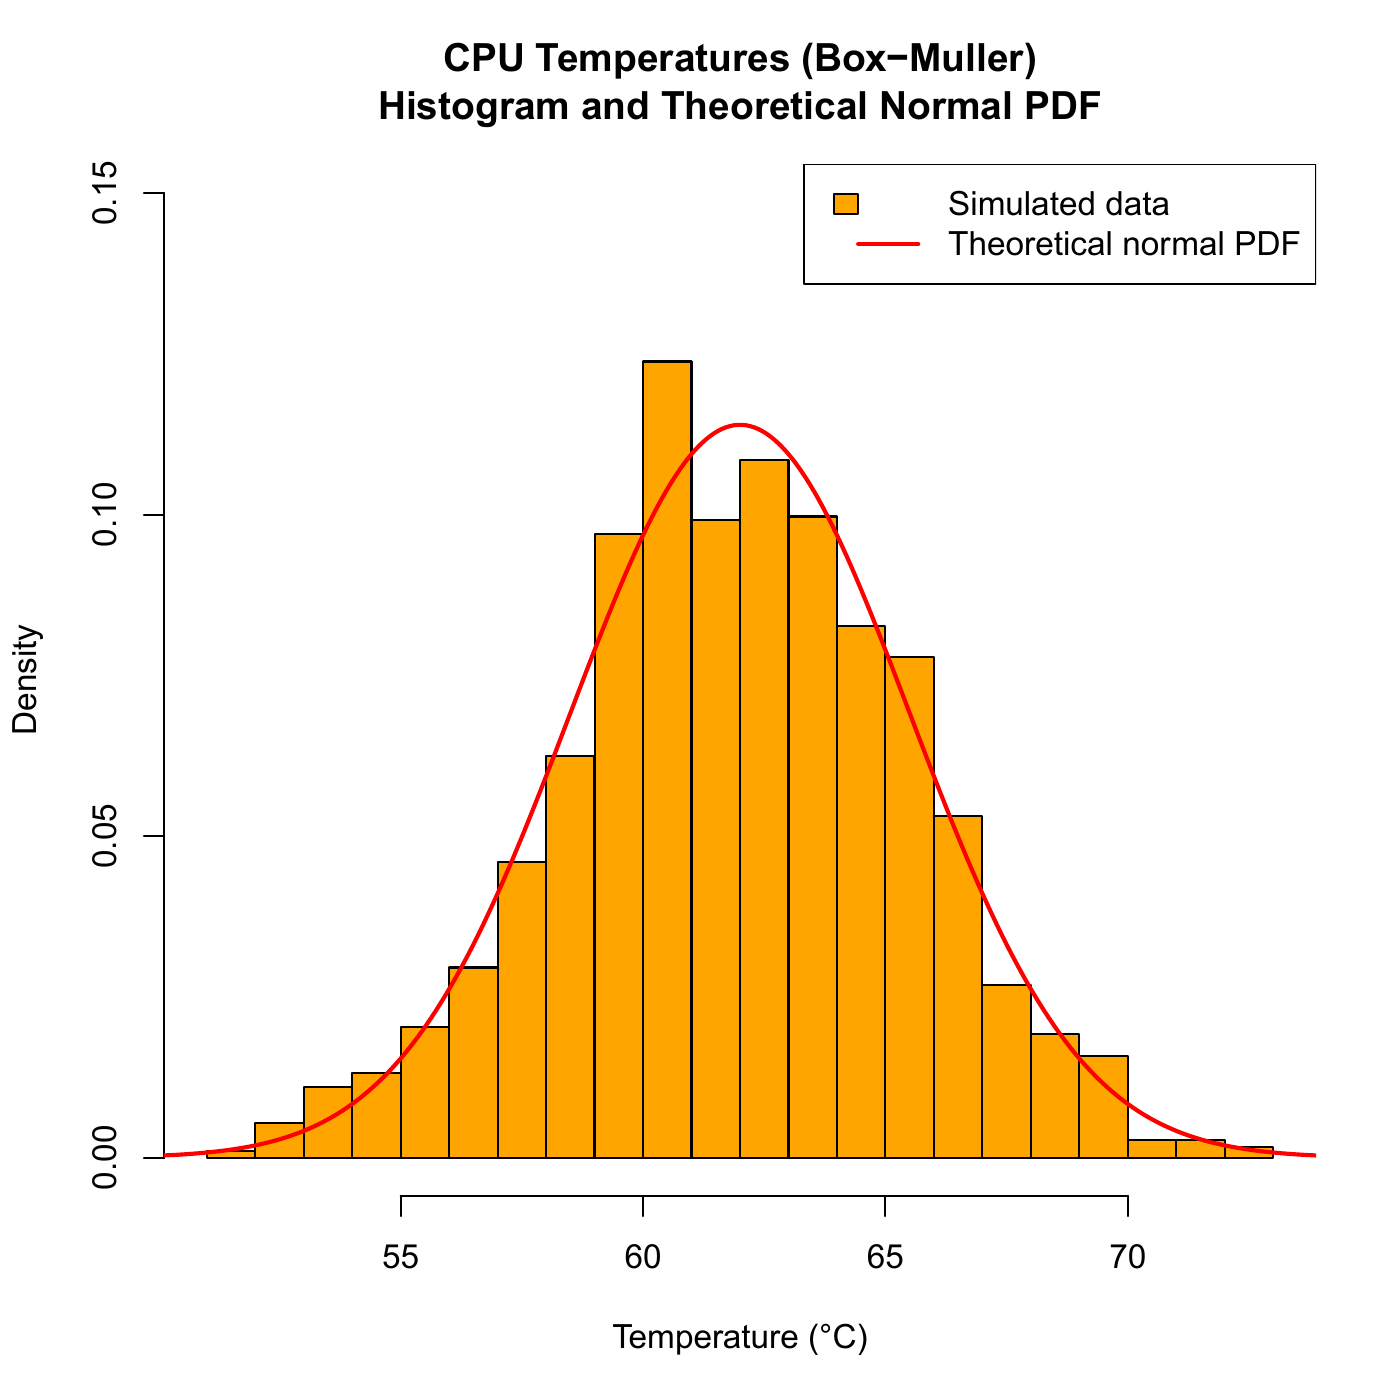
\includegraphics[width=\textwidth]{imagens/hist_bm_q3.png}
    \caption{Simulação por Box-Muller (\texttt{temp\_bm})}
    \label{fig:q3-hist-bm}
\end{subfigure}
\hfill
\begin{subfigure}{0.48\textwidth}
    \centering
    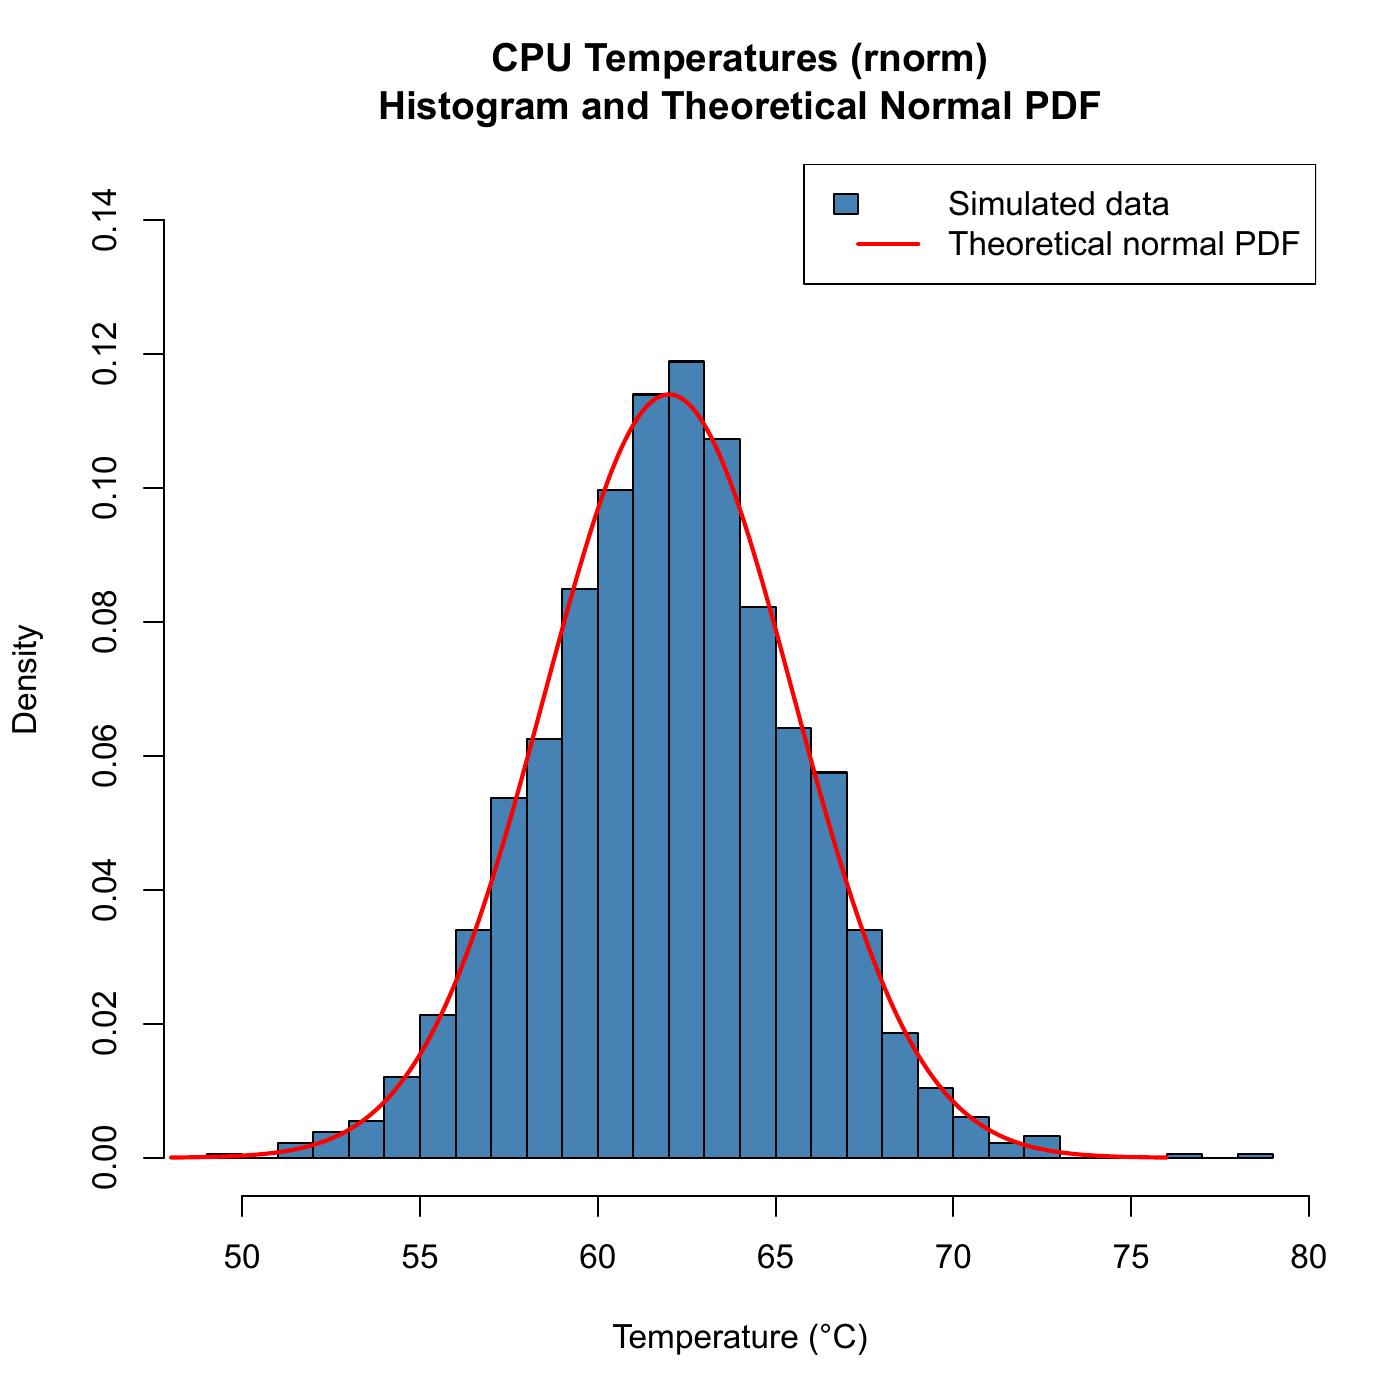
\includegraphics[width=\textwidth]{imagens/hist_rnorm_q3.png}
    \caption{Simulação por \texttt{rnorm} (\texttt{temp\_r})}
    \label{fig:q3-hist-rnorm}
\end{subfigure}
\caption{Histogramas em escala de densidade das $n_T = 1\,825$ temperaturas simuladas da CPU, sobrepostos à PDF teórica da distribuição $N(62;\; 3{,}5^{2})$}
\label{fig:q3-hist}
\end{figure}

Visualmente, ambos os histogramas exibem o formato unimodal e simétrico em sino característico da distribuição normal, centrados em torno de $62\,^\circ\text{C}$ e acompanhando de perto a curva vermelha da densidade teórica tanto na região central quanto nas caudas. No histograma gerado por Box-Muller (Figura~\ref{fig:q3-hist}a), a barra mais alta ocorre no intervalo $[60;\; 61]\,^\circ\text{C}$ (densidade $\approx 0{,}1238$, ligeiramente acima do pico teórico de $0{,}1140$), acompanhada de pequena depressão em $[61;\; 62]\,^\circ\text{C}$ — flutuações pontuais típicas de uma amostra finita particionada em classes de $1\,^\circ\text{C}$. No histograma gerado por \texttt{rnorm} (Figura~\ref{fig:q3-hist}b), o pico localiza-se em $[62;\; 63]\,^\circ\text{C}$ (densidade $\approx 0{,}1189$) e a aderência visual na região central é muito próxima da curva teórica; na cauda direita, notam-se duas barras isoladas de altura mínima em $[76;\; 77]\,^\circ\text{C}$ e $[78;\; 79]\,^\circ\text{C}$, correspondentes às duas observações extremas da amostra ($76{,}76\,^\circ\text{C}$ e $78{,}03\,^\circ\text{C}$), que ampliam o eixo horizontal sem comprometer a distribuição global.

Para complementar a inspeção visual, a Tabela~\ref{tab:q3-regra} compara as proporções empíricas de observações dentro de 1, 2 e 3 desvios padrão em torno da média teórica $\mu = 62\,^\circ\text{C}$ (variáveis \texttt{within\_bm} e \texttt{within\_r}) com a regra empírica da distribuição normal.

\begin{table}[H]
\centering
\caption{Proporção de temperaturas simuladas dentro de 1, 2 e 3 desvios padrão da média teórica ($\mu = 62\,^\circ\text{C}$, $\sigma = 3{,}5\,^\circ\text{C}$)}
\label{tab:q3-regra}
\begin{tabular}{lccc}
\hline
\textbf{Intervalo} & \textbf{Teórico} & \textbf{Box-Muller} & \textbf{\texttt{rnorm}} \\
\hline
$\mu \pm 1\sigma = [58{,}5;\; 65{,}5]\,^\circ\text{C}$ & 0,6827 (68,27\%) & 0,6816 (68,16\%) & 0,6707 (67,07\%) \\
$\mu \pm 2\sigma = [55{,}0;\; 69{,}0]\,^\circ\text{C}$ & 0,9545 (95,45\%) & 0,9463 (94,63\%) & 0,9529 (95,29\%) \\
$\mu \pm 3\sigma = [51{,}5;\; 72{,}5]\,^\circ\text{C}$ & 0,9973 (99,73\%) & 0,9984 (99,84\%) & 0,9984 (99,84\%) \\
\hline
\end{tabular}
\end{table}

Em ambos os conjuntos, as proporções empíricas reproduzem fielmente os referenciais teóricos de $68{,}27\%$, $95{,}45\%$ e $99{,}73\%$, com diferenças inferiores a $1{,}2$ ponto percentual em todos os intervalos. Em conjunto com os resultados da Tabela~\ref{tab:q3-resumo} e dos histogramas da Figura~\ref{fig:q3-hist}, conclui-se que a implementação própria da transformação de Box-Muller produz amostras estatística e visualmente equivalentes às do gerador nativo \texttt{rnorm}, representando adequadamente a distribuição normal $N(62;\; 3{,}5^{2})$ adotada para a temperatura da CPU.

\clearpage

\section{Questão 4}

% Introdução e desenvolvimento da questão.

\subsection{Ponto 1 -- Descrição}

% Desenvolvimento.

\subsection{Ponto 2 -- Descrição}

% Desenvolvimento.

\subsection{Ponto 3 -- Descrição}

% Desenvolvimento.

\subsection{Ponto 4 -- Descrição}

% Desenvolvimento.

% ===================== REFERÊNCIAS =====================
\clearpage
\section*{Referências}
\addcontentsline{toc}{section}{Referências}

\begin{enumerate}[label={[\arabic*]}, leftmargin=*, itemsep=8pt]
    % Ajeitar referêcias depois, essas são do hw passado e que podemos utilizar
    \item \textbf{UNIVERSIDADE FEDERAL DO CEARÁ (UFC)}. \textit{Slides das Aulas da Disciplina de Estatística para Engenharia (TI0111) -- Aulas L01 a L04}: Introdução à Estatística Descritiva, Medidas de Tendência Central, Dispersão, Separatrizes (Quartis e IQR), Gráficos (Boxplot e Histograma) e Associação Bivariada. Fortaleza, 2026.
    
    \item \textbf{R CORE TEAM}. \textit{R: A Language and Environment for Statistical Computing}. R Foundation for Statistical Computing, Vienna, Austria, 2024. Disponível em: \url{https://www.R-project.org/}.
    
    \item \textbf{R DOCUMENTATION}. \textit{The R Stats Package: Functions for Statistical Distributions and Calculations (\texttt{quantile}, \texttt{cor}, \texttt{summary}, \texttt{sd})}. R Foundation for Statistical Computing, 2024.
    
    \item \textbf{WICKHAM, H.; GROLEMUND, G.} \textit{R for Data Science: Import, Tidy, Transform, Visualize, and Model Data}. Sebastopol: O'Reilly Media, 2017.
\end{enumerate}

\end{document}
